% Data

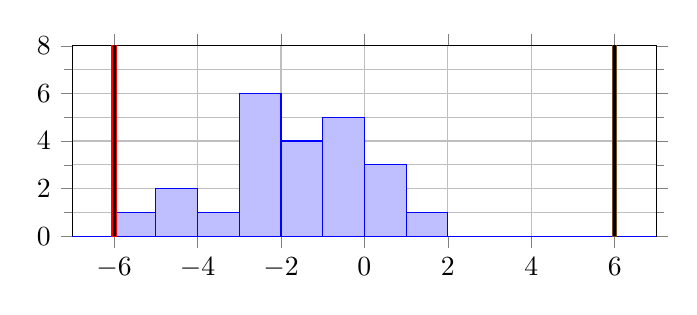
\begin{tikzpicture}
\begin{axis}[
height=4cm,
width=9cm,
%            ybar interval,      % <-- this causes the `xticks' to be centered
ymin= 0, ymax=8,
xmin=-7, xmax=7,
grid=both,
minor y tick num=1,
%yminorgrids=true,
tick align=outside, % <-- this positions the ticks "outside"
]
\addplot+ [
ybar interval,
mark=none,
fill=blue!25,   % fill the bars again
] coordinates {

	(-7,0)	%
	(-6,1)	%1
	(-5,2)	%11
	(-4,1)	%1
	(-3,6)	%111111
	(-2,4)	%1111
	(-1,5)	%11111
	 (0,3)	%111
	 (1,1)	%1
	 (2,0)	%
	 (3,0)	%
	 (4,0)	%
	 (5,0)	%
	 (6,0)	%
	 (7,0)	%

};

\addplot+ [
ybar interval,
mark=none,
fill=black,   % fill the bars again
] coordinates {
	(-6.05,16) 
	(-5.95,16) 
};

\addplot+ [
ybar interval,
mark=none,
fill=black,   % fill the bars again
] coordinates {
	(6.05,16) 
	(5.95,16) 
};
\end{axis}

\end{tikzpicture}